%% ============================================================================
%% Capítulo 6 --- O Arcabouço de Decisão Validado
%%
%% Fontes (auditadas; nenhum número sem origem em artefato versionado):
%%   - dissertation/cap6-framework.md ............ prosa auditada; tabela de
%%     regret @11/@14 (idêntica à da AI-1)
%%   - latex/ai1/main.tex, seção "The Validated Decision Framework" ........
%%     formulação final auditada (taxa de acerto (\emph{hit-rate}) 0,11 vs 0,44 @11 e 0,72 vs 0,78
%%     @14; explicação do empate árvore/FM; rice1976; herre2026) --- prevalece
%%     sobre o rascunho em caso de divergência
%%   - docs/desenho-melhorias-finais.md, seção E2 .... pré-registro do regret
%%     multicritério ponderado (05/10/2026, antes da execução)
%%   - results/aggregated/lodo_weighted_regret.csv ... dados do E2; medianas e
%%     médias por política × w recomputadas do CSV (pandas) em 05/10/2026
%%   - scripts/lodo_validation.py; results/aggregated/lodo_validation{,_14}.csv
%%
%% Figuras (copiadas para dissertacao/images/ em 05/10/2026):
%%   - images/decision_matrix.png ........ de results/figures/decision_matrix.png
%%   - images/lodo_weighted_regret.pdf ... de results/figures/lodo_weighted_regret.pdf
%%   - images/decision_flowchart_14.pdf .. versao PT gerada por scripts/figures_ai1_display.py
%%     (gerada por scripts/figures_ai1_display.py)
%% ============================================================================

\chapter{O Arcabouço de Decisão Validado}
\label{chap:framework}

Este capítulo tem como objetivo elevar o arcabouço de decisão de
descritivo a validado, por meio de três estudos sobre os mesmos 18
conjuntos de dados do benchmark: um resultado negativo, em que o
roteamento por meta-características não generaliza sob validação
\emph{leave-one-dataset-out}; um resultado positivo, em que a política
fixa ``\emph{foundation model} primeiro'' é regret-ótima na métrica
primária; e um experimento pré-registrado de \emph{regret} multicritério
ponderado, que localiza o peso de latência em que essa recomendação se
inverte --- basta deslocar 10--20\% do peso da acurácia para a latência.
O arcabouço resultante é um fluxograma de quatro restrições verificáveis
\emph{a priori}, no qual a primeira pergunta --- latência --- é agora
quantitativamente justificada.

\section{Do descritivo ao validado}
\label{sec:descritivo-validado}

O benchmark multicritério do Capítulo~\ref{chap:benchmark} produz, por
construção, um artefato prático: dado um problema novo, que modelo usar?
A primeira versão do arcabouço respondia com dois instrumentos
descritivos. O primeiro é a matriz multicritério, que resume a posição
de cada um dos 14 modelos em seis critérios medidos no benchmark ---
desempenho, custo de treino, custo de ajuste de hiperparâmetros,
latência de inferência, robustez e interpretabilidade. A
Figura~\ref{fig:decision-matrix} apresenta essa matriz, com escores de 1
a 3 estrelas computados do benchmark (3 = melhor; tom mais escuro =
melhor), e sua leitura motiva todo o restante do capítulo.

\begin{figure}[htb]
\centering
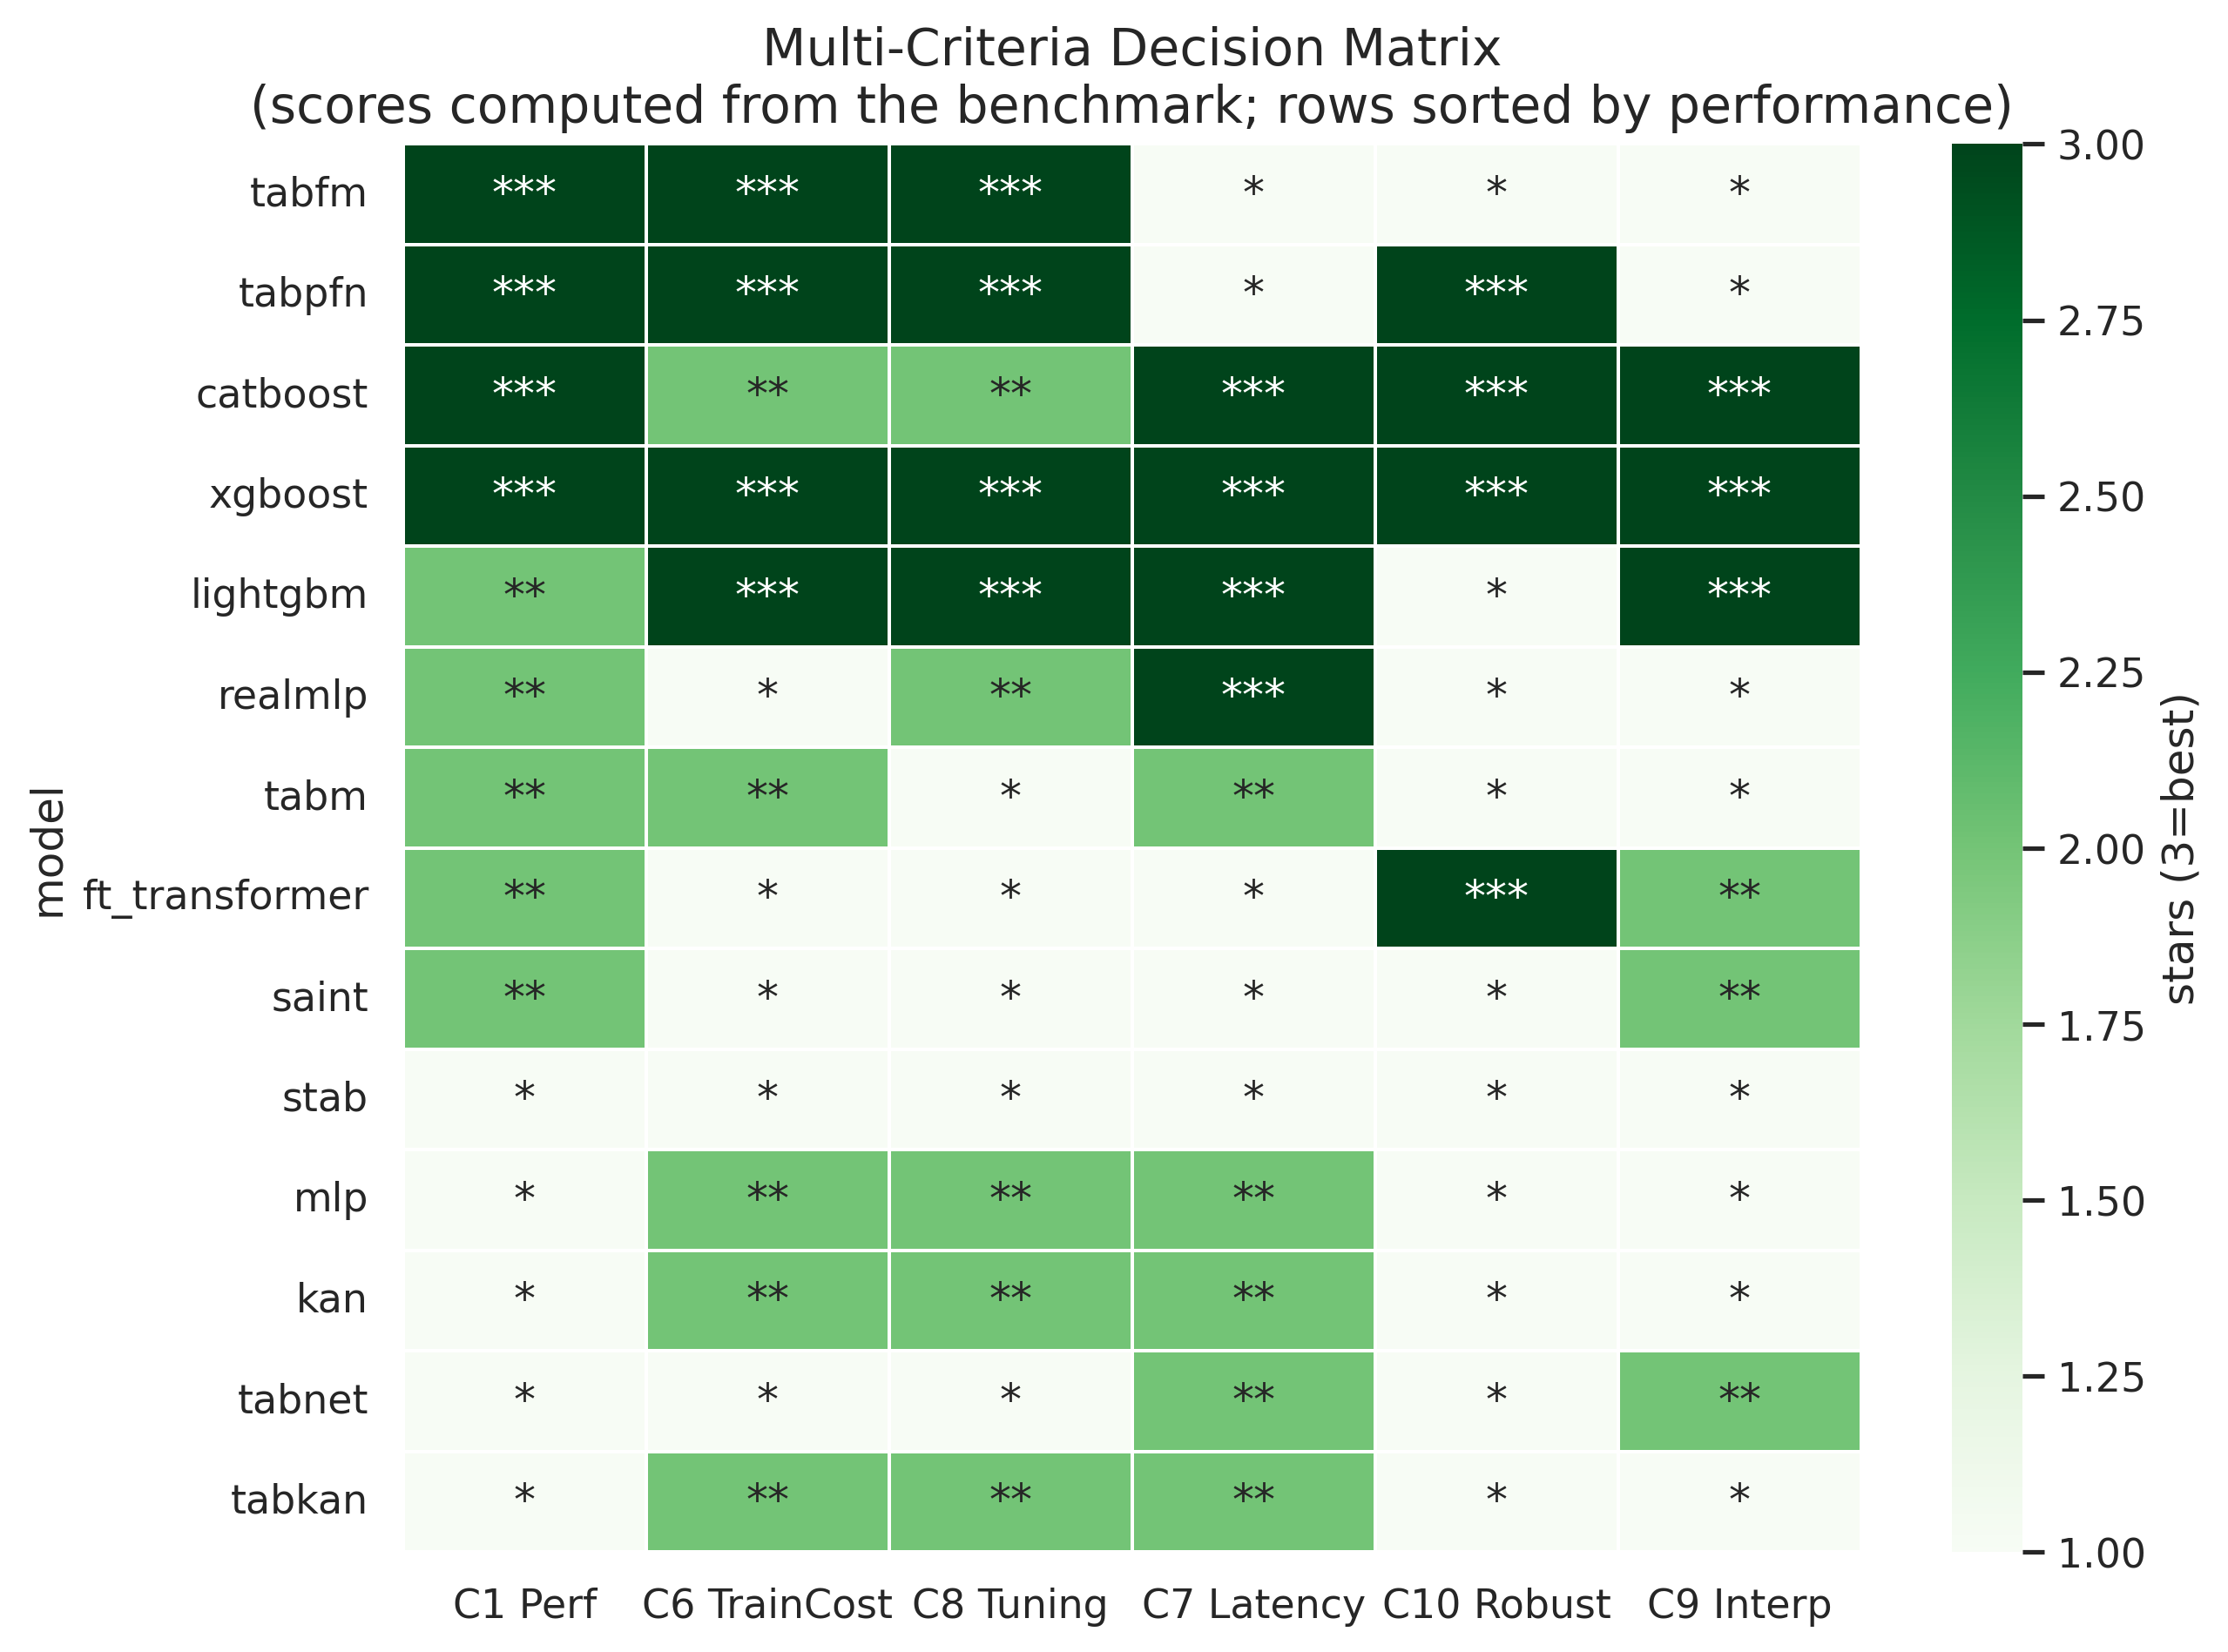
\includegraphics[width=0.92\linewidth]{images/decision_matrix.png}
\caption{Matriz de decisão multicritério dos 14 modelos (linhas,
ordenadas por desempenho) em seis critérios (colunas; rótulos internos da
figura em inglês). Fonte: \texttt{results/figures/decision\_matrix.png}.}
\label{fig:decision-matrix}
\end{figure}

A matriz torna visível o padrão central: as linhas do topo (foundation
models) e as do meio (GBDTs) têm perfis \emph{complementares}, não
ordenáveis --- o que é ótimo em desempenho é fraco em latência, e
vice-versa. O segundo instrumento, o fluxograma orientado a restrições
(apresentado em sua forma final na Seção~\ref{sec:arcabouco-resultante}),
codifica esse compromisso como uma sequência de perguntas verificáveis
antes de qualquer treino.

Ambos os instrumentos, porém, são descritivos: resumem o que o benchmark
mediu, mas não foram testados contra conjuntos que não participaram de
sua construção. Um arcabouço de recomendação que nunca foi exposto a
esse teste está sujeito à mesma crítica de \emph{overclaiming} que
atinge parte da literatura de recomendação de algoritmos. Este capítulo
eleva o arcabouço de descritivo a \textbf{validado} com dois resultados
complementares --- um negativo (o que o arcabouço \emph{não} deve tentar
fazer) e um positivo (a política que os dados sustentam) --- e, em
seguida, com um terceiro estudo, pré-registrado, que estende a validação
ao cenário multicritério.

\section{O resultado negativo: roteamento por meta-características não
generaliza}
\label{sec:resultado-negativo}

A literatura de meta-learning, que remonta ao problema de seleção de
algoritmos \citep{rice1976}, sugere um caminho sedutor: prever o
algoritmo vencedor a partir de meta-características do conjunto de dados ---
tamanho, dimensionalidade, desbalanceamento, fração de atributos
categóricos. Se funcionasse, o arcabouço de decisão seria um modelo
preditivo, não um fluxograma. Testamos essa promessa com o protocolo
honesto disponível para $N{=}18$ conjuntos: validação
\emph{leave-one-dataset-out} (LODO), em que uma árvore de decisão de
profundidade 2 --- o mesmo modelo ilustrativo da Figura~2.1, no
Capítulo~\ref{chap:fundamentacao} --- é treinada nos demais 17 conjuntos para
prever a família vencedora do conjunto excluído, repetindo-se o
procedimento para cada um dos 18.

O resultado contraria a expectativa criada pela literatura --- e por
isso o reportamos com o protocolo à vista. No estudo com 11 modelos
(o núcleo de 11 modelos do estudo original), a árvore atinge \textbf{taxa de acerto de 0,11 contra
0,44 do \emph{baseline} de classe majoritária}; no estudo com 14 modelos
(incluindo a geração 2026), 0,72 contra 0,78 do \emph{baseline}. Em nenhuma
das duas configurações o roteador aprendido supera a regra trivial
``preveja sempre a família que mais vence''. Investigado o porquê, a
atribuição é direta: com $N{=}18$ conjuntos, cada rodada do LODO
treina com 17 exemplos --- uma amostra em que qualquer partição por
meta-características é dominada pelo ruído das reversões individuais, e em
que o preço de errar uma folha é alto. O resumo honesto é este:
aprender o roteamento por meta-características não é viável sob LODO com essa
classe de modelo nesta escala de $N$ --- e afirmar isso sob um protocolo
explícito protege o arcabouço da crítica de \emph{overclaiming}
mencionada acima. A árvore permanece no trabalho como \emph{ilustração
descritiva da estrutura} das reversões entre famílias, jamais como
preditor.

Evidência independente e contemporânea aponta na mesma direção:
abordagens globais baseadas em meta-características não são robustas o
suficiente para explicar ou selecionar entre modelos da era dos
\emph{foundation models} tabulares \citep{herre2026}. A convergência entre
nosso protocolo LODO e um estudo externo, com metodologia distinta,
reforça que o resultado negativo não é um artefato da nossa amostra de
conjuntos.

\emph{Roteamento por meta-características não generaliza sob LODO.}
Com $N{=}18$ conjuntos, um roteador aprendido (árvore de profundidade
2) não supera o \emph{baseline} de classe majoritária em nenhuma das duas
gerações de modelos (0,11 vs.\ 0,44 com 11 modelos; 0,72 vs.\ 0,78 com
14). O arcabouço de decisão não deve conter um preditor de família
vencedora --- conclusão corroborada por evidência independente
\citep{herre2026}.

\section{O resultado positivo: a política ``FM primeiro'' e sua
evolução}
\label{sec:resultado-positivo}

Se o roteamento aprendido não funciona, a alternativa natural são
\emph{políticas fixas}: recomendar sempre a mesma família,
independentemente do conjunto. Para compará-las, usamos a métrica de
\textbf{regret normalizado} sobre a métrica primária de cada conjunto:
0 significa que a família recomendada contém o melhor modelo do
conjunto; 1, que contém apenas o pior. A
Tabela~\ref{tab:regret-lodo} resume o \emph{regret} das quatro políticas ---
a árvore sob LODO e as três políticas fixas --- nos dois estudos; as
linhas da árvore e da política sempre-FM agregam sobre os 17 conjuntos em
que a família FM participa (\texttt{helena} é excluída por limite
arquitetural de 100 classes), e as linhas sempre-GBDT e sempre-DL, sobre
todos os 18.

\begin{table}[htb]
\centering
\caption{Regret normalizado das políticas de recomendação sob LODO, nos
estudos com 11 e com 14 modelos (\textbf{negrito} = melhor política da
coluna). Fonte: \texttt{results/aggregated/lodo\_validation\{,\_14\}.csv}.}
\label{tab:regret-lodo}
\small
\begin{tabular}{lcccc}
\toprule
Política & média @11 & mediana @11 & média @14 & mediana @14 \\
\midrule
Árvore (LODO)      & 0,228 & 0,145 & 0,051 & 0,000 \\
Sempre-GBDT        & 0,249 & 0,168 & 0,305 & 0,291 \\
Sempre-DL          & 0,189 & 0,132 & 0,313 & 0,349 \\
\textbf{Sempre-FM} & \textbf{0,115} & \textbf{0,018} & \textbf{0,021} &
\textbf{0,000} \\
\bottomrule
\end{tabular}
\end{table}

Três leituras emergem da tabela. Primeiro, já no núcleo de 11 modelos do estudo original,
``usar o \emph{foundation model} por padrão'' era a melhor política fixa
(\emph{regret} médio 0,115; mediano 0,018). Segundo, com a geração 2026, o
\emph{regret} mediano da política cai a \textbf{zero}: em metade ou mais dos
conjuntos, a família FM contém o melhor modelo, ponto. A pergunta
``qual família vence?'' se dissolve --- e com ela o valor de qualquer
roteador de desempenho. Terceiro, o aparente empate entre a árvore e a
política sempre-FM na mediana @14 (ambas 0,000) merece explicação, e
ela desfaz o empate: com 14 modelos, a árvore aprende a prever a
família FM em quase todos os conjuntos, colapsando na política fixa ---
mas mantendo taxa de acerto \emph{abaixo} do \emph{baseline} de classe majoritária
(Seção~\ref{sec:resultado-negativo}). A política fixa atinge o mesmo
\emph{regret} sem esse modo de falha; o colapso da árvore é mais um sintoma de
que não há estrutura aprendível, não uma vitória do roteador.

\emph{``Foundation model primeiro'' é a política regret-ótima na
métrica primária.} Na geração 2026, a política fixa sempre-FM atinge
\emph{regret} médio 0,021 e mediano 0,000 sob LODO --- nenhuma política
aprendida ou fixa a supera. A recomendação de desempenho deixou de
depender do conjunto de dados; a ressalva é que esse resultado vale
para a métrica primária isolada, questão que a próxima seção enfrenta.

\section{Regret multicritério ponderado: quando a recomendação vira}
\label{sec:regret-ponderado}

O resultado positivo da seção anterior tem uma limitação declarada
desde o artigo AI-1: o \emph{regret} é calculado sobre a métrica primária,
não sobre combinações multicritério ponderadas por preferências do
usuário. A limitação não é cosmética. O Capítulo~\ref{chap:benchmark}
mostrou que o líder de acurácia custa 4--5 ordens de magnitude mais
para servir que um GBDT; um praticante cuja função de utilidade pondere
acurácia \emph{e} custo de inferência pode, legitimamente, chegar a
outra recomendação. Esta seção fecha essa lacuna com o experimento E2,
pré-registrado em \texttt{docs/desenho-melhorias-finais.md}
(05/10/2026, antes da execução, conforme o contrato de conduta do
programa de pesquisa): a política ``FM primeiro'' continua regret-ótima
quando a métrica de decisão pondera acurácia e custo?

\subsection{Desenho pré-registrado}
\label{sec:e2-desenho}

O desenho define um score multicritério por modelo$\times$conjunto:
\begin{equation}
S \;=\; w \cdot r_{\text{acc}} \;+\; (1-w) \cdot r_{\text{lat}},
\label{eq:score-ponderado}
\end{equation}
em que $r_{\text{acc}}$ é o rank normalizado em $[0,1]$ do modelo na
métrica primária do conjunto, $r_{\text{lat}}$ é o rank normalizado da
latência de inferência, e $w \in \{1{,}0;\, 0{,}9;\, \ldots;\, 0{,}0\}$
varre o espectro de preferências --- de ``só acurácia importa''
($w{=}1$) a ``só latência importa'' ($w{=}0$). Para cada valor de $w$,
calcula-se o \emph{regret} normalizado de cada política fixa exatamente como
no estudo original: 0 se a família recomendada contém o modelo de
melhor score $S$ no conjunto; 1 se contém apenas o pior.\footnote{As
quatro políticas do pré-registro estão no artefato
(\texttt{results/aggregated/lodo\_weighted\_regret.csv}): a árvore-LODO
é avaliada pela recomendação por conjunto armazenada no estudo original
(\texttt{lodo\_validation\_14.csv}), sem reajuste --- ela foi treinada
para prever o vencedor de \emph{acurácia} e aqui é pontuada sob o score
ponderado. O resultado antecipa a Seção~\ref{sec:resultado-negativo}:
a árvore nunca supera a melhor política fixa em nenhum $w$ e colapsa na
política sempre-FM nos pesos altos (mediana 0{,}000 apenas em
$w \geq 0{,}9$).}
Os $N$s espelham os da Tabela~\ref{tab:regret-lodo}: 18 conjuntos para
as políticas sempre-GBDT e sempre-DL, 17 para sempre-FM
(\texttt{helena} excluída por limite arquitetural). A hipótese
pré-registrada H-W1 afirma: existe $w^{*} < 1$ a partir do qual
``sempre-GBDT'' passa a ter \emph{regret} mediano menor que ``sempre-FM'' ---
o que tornaria o fluxograma (pergunta 1 = latência) a forma correta da
política, e não um refinamento cosmético.

Uma limitação do desenho foi declarada no próprio pré-registro e deve
ser repetida aqui: a latência usa como \emph{proxy} a medição
padronizada no conjunto \texttt{adult} --- a única disponível para os 14
modelos sob protocolo idêntico. A latência relativa entre modelos é
aproximadamente estável entre conjuntos para GBDTs e modelos de deep
learning; para \emph{foundation models}, porém, ela cresce com o tamanho do
contexto, de modo que o proxy é conservador a favor dos FMs em
conjuntos pequenos e contra eles em conjuntos grandes. As conclusões
desta seção devem ser lidas com essa ressalva.

\subsection{Resultados: o cruzamento}
\label{sec:e2-resultados}

A Figura~\ref{fig:lodo-weighted} mostra o que a
Tabela~\ref{tab:regret-lodo} não pode mostrar: como o \emph{regret} de cada
política evolui à medida que o peso se desloca da acurácia para a
latência --- o painel esquerdo traz a mediana e o direito, a média sobre
os conjuntos.

\begin{figure}[htb]
\centering
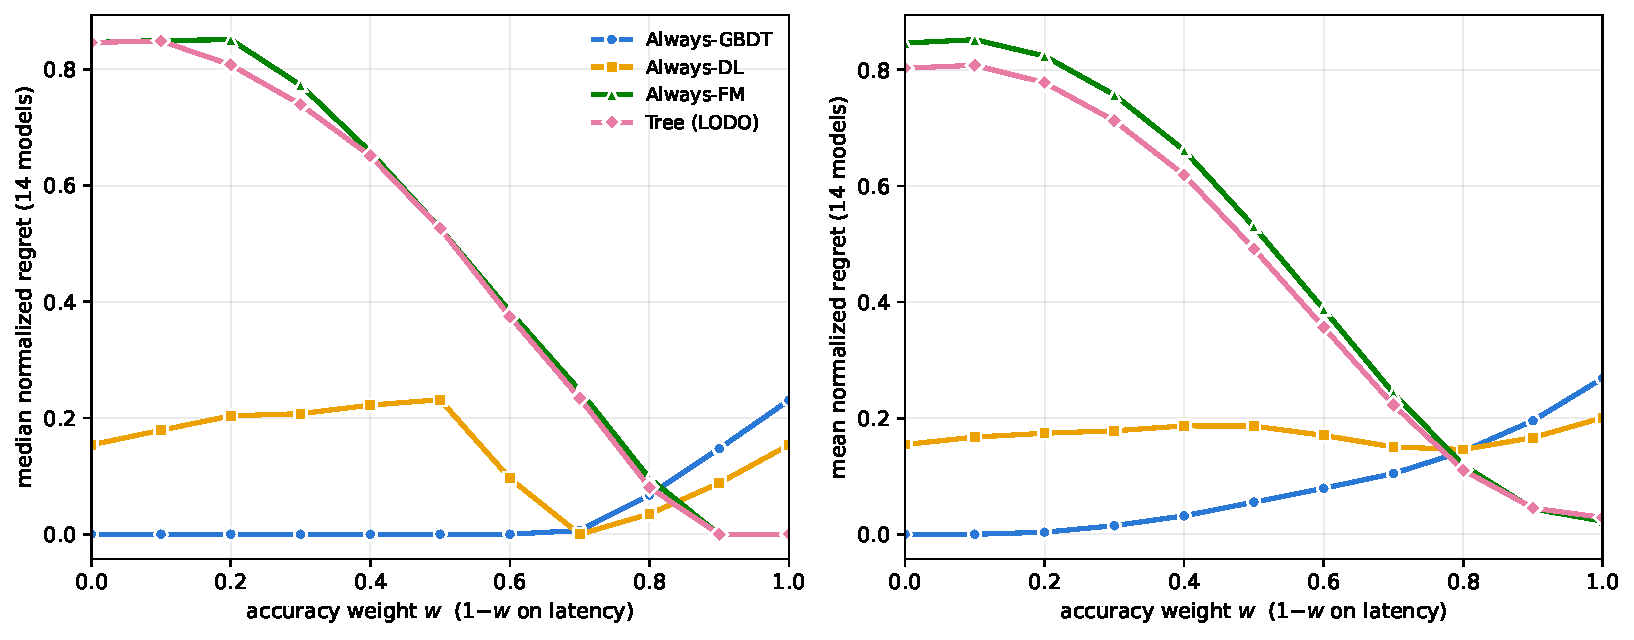
\includegraphics[width=\linewidth]{images/lodo_weighted_regret.pdf}
\caption{Regret multicritério ponderado das três políticas fixas em
função do peso da acurácia $w$ (Eq.~\ref{eq:score-ponderado}; experimento
E2, estudo com 14 modelos). Fonte:
\texttt{results/aggregated/lodo\_weighted\_regret.csv}.}
\label{fig:lodo-weighted}
\end{figure}

A Tabela~\ref{tab:weighted-regret} dá os valores exatos da mediana em
pontos selecionados da varredura, para que cada número citado a seguir
tenha origem inspecionável.

\begin{table}[htb]
\centering
\caption{Regret normalizado mediano das três políticas fixas em função do
peso da acurácia $w$ (estudo com 14 modelos; \textbf{negrito} = melhor
política da coluna). Fonte:
\texttt{results/aggregated/lodo\_weighted\_regret.csv} (medianas
recomputadas do artefato).}
\label{tab:weighted-regret}
\small
\begin{tabular}{lccccccc}
\toprule
Política & $w{=}1{,}0$ & $w{=}0{,}9$ & $w{=}0{,}8$ & $w{=}0{,}7$ &
$w{=}0{,}6$ & $w{=}0{,}5$ & $w{=}0{,}0$ \\
\midrule
Sempre-GBDT & 0,231 & 0,147 & 0,067 & 0,007 & \textbf{0,000} &
\textbf{0,000} & \textbf{0,000} \\
Sempre-DL   & 0,154 & 0,088 & \textbf{0,035} & \textbf{0,000} & 0,096 &
0,232 & 0,154 \\
Sempre-FM   & \textbf{0,000} & \textbf{0,000} & 0,096 & 0,248 & 0,383 &
0,526 & 0,846 \\
\bottomrule
\end{tabular}
\end{table}

A leitura conjunta da figura e da tabela estabelece três fatos.
Primeiro, \textbf{a hipótese H-W1 é confirmada, e o cruzamento é
precoce}: na grade de varredura, a política sempre-FM só mantém \emph{regret}
mediano zero em $w \in \{0{,}9;\, 1{,}0\}$. Já em $w^{*}{=}0{,}8$ ---
apenas 20\% do peso na latência --- tanto sempre-GBDT (0,067) quanto
sempre-DL (0,035) têm \emph{regret} mediano menor que sempre-FM (0,096); o
cruzamento, portanto, ocorre entre $w{=}0{,}9$ e $w{=}0{,}8$. Pela
média (painel direito da Figura~\ref{fig:lodo-weighted}), o quadro é
ligeiramente mais favorável aos FMs: sempre-FM ainda é a melhor
política em $w{=}0{,}8$ (0,119 contra 0,143 do GBDT e 0,146 do DL) e
só perde em $w{=}0{,}7$ (0,243 contra 0,105 do GBDT). Segundo, a partir
de $w \leq 0{,}6$, ``sempre-GBDT'' tem \emph{regret} mediano exatamente zero ---
assim que a latência domina a função de utilidade, a família GBDT
contém o melhor modelo em metade ou mais dos conjuntos, espelhando no
extremo oposto o que a família FM faz em $w{=}1$. Terceiro, no extremo
$w{=}0$ (só latência), o \emph{regret} mediano de sempre-FM atinge 0,846: a
família que contém o melhor modelo em acurácia contém quase o pior em
custo de inferência, o retrato numérico do compromisso que a
Figura~\ref{fig:decision-matrix} mostrava em estrelas.\footnote{Em
$w{=}1{,}0$, o score da Eq.~\ref{eq:score-ponderado} reduz-se ao rank
da métrica primária; os valores diferem marginalmente dos da
Tabela~\ref{tab:regret-lodo} (\emph{regret} médio de sempre-FM 0,023 aqui
contra 0,021 lá) porque o \emph{regret} do estudo original é normalizado na
escala da métrica primária, e o de E2, na escala de ranks. As medianas
coincidem em 0,000.}

A interpretação pré-fixada no registro do experimento aplica-se
diretamente: qualquer que fosse $w^{*}$, o resultado enriqueceria o
arcabouço ao quantificar o \emph{trade-off} que ele já codificava
qualitativamente. O valor encontrado --- cruzamento entre $w{=}0{,}9$ e
$w{=}0{,}8$ pela mediana --- faz mais que enriquecer: ele explica
\emph{por que a primeira pergunta do fluxograma é a latência}. Se a
recomendação só se sustentasse com 99\% do peso em acurácia, a pergunta
de latência seria um detalhe de borda; como ela vira com 10--20\% de
peso na latência, a pergunta é o eixo da decisão. O fluxograma da
próxima seção não é uma heurística decorativa em torno de uma política
única --- é a codificação da fronteira que a
Figura~\ref{fig:lodo-weighted} mede. Dito de outro modo: antes de E2,
sabíamos que a latência \emph{importava} (a matriz da
Figura~\ref{fig:decision-matrix} já o mostrava em estrelas); depois de
E2, sabemos \emph{quanto} ela precisa importar para mudar a resposta ---
e a resposta é: pouco.

\emph{A recomendação ``FM primeiro'' inverte-se com 10--20\% de
peso na latência.} Sob o score ponderado
$S = w \cdot r_{\text{acc}} + (1-w) \cdot r_{\text{lat}}$, a política
sempre-FM só é regret-ótima na mediana para $w \geq 0{,}9$; em
$w{=}0{,}8$ já é superada por sempre-GBDT e sempre-DL, e para
$w \leq 0{,}6$ ``sempre-GBDT'' tem \emph{regret} mediano zero. A ressalva
acompanha o achado: a latência usa o proxy padronizado do
\texttt{adult}, conservador a favor dos FMs em conjuntos pequenos e
contra eles em grandes.

\section{O arcabouço resultante: decisão por restrições}
\label{sec:arcabouco-resultante}

Os três estudos convergem para uma mesma conclusão: o que resta de
informativo na decisão --- e o que o fluxograma sempre codificou --- são
\textbf{restrições verificáveis \emph{a priori}}, não predições de
desempenho. A Figura~\ref{fig:flowchart-14} apresenta o fluxograma
validado na sua forma final, com os 14 modelos do estudo completo.

\begin{figure}[htb]
\centering
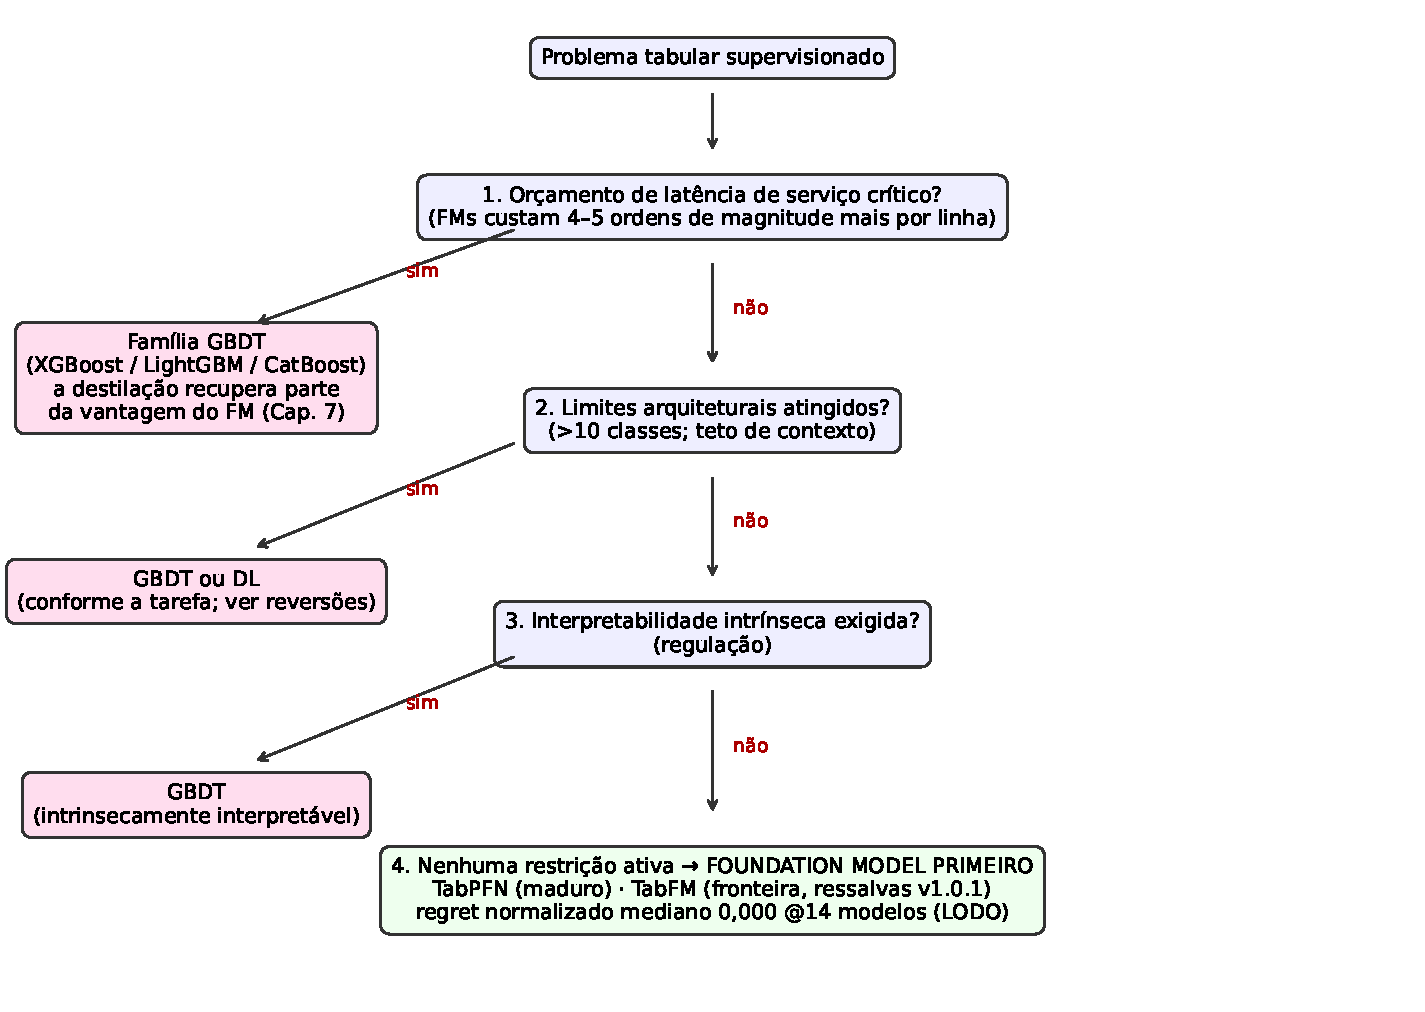
\includegraphics[width=0.88\linewidth]{images/decision_flowchart_14_pt.pdf}
\caption{Fluxograma de decisão validado, estudo com 14 modelos: cada
losango é uma restrição verificável \emph{a priori}. Gerado por
\texttt{scripts/figures\_ai1\_display.py}.}
\label{fig:flowchart-14}
\end{figure}

As quatro restrições, na ordem em que o fluxograma as verifica:

\begin{enumerate}
  \item \textbf{Latência e custo de inferência.} O líder de acurácia
    custa 4--5 ordens de magnitude mais para servir
    (Capítulo~\ref{chap:benchmark}); se o orçamento de latência é de
    microssegundos, a família FM está excluída na forma nativa. O
    experimento E2 quantifica por que esta é a primeira pergunta: a
    recomendação inverte com apenas 10--20\% do peso na latência
    (Seção~\ref{sec:regret-ponderado}). Recuperar a família FM dentro
    desse orçamento é precisamente o objeto do
    Capítulo~\ref{chap:destilacao}.
  \item \textbf{Limites arquiteturais.} Mais de 10 classes (limite do
    TabFM) ou estouro do limite de contexto são exclusões estruturais
    objetivas --- o caso \texttt{helena} (100 classes) no próprio
    benchmark.
  \item \textbf{Interpretabilidade intrínseca exigida.} Quando a
    regulação do domínio exige modelos intrinsecamente interpretáveis,
    a recomendação são os GBDTs --- a única família com perfil
    simultaneamente forte em latência e interpretabilidade na matriz da
    Figura~\ref{fig:decision-matrix}.
  \item \textbf{Nenhuma restrição ativa.} Aplica-se o \emph{default}
    regret-ótimo: \emph{foundation model}, com o TabPFN \citep{hollmann2025}
    como opção madura e o TabFM \citep{tabfm2026} como fronteira, com
    as ressalvas de maturidade discutidas no
    Capítulo~\ref{chap:benchmark}.
\end{enumerate}

A validação por \emph{regret} confirma que essas quatro perguntas capturam o
essencial: as restrições são o \emph{conteúdo informativo real} da
decisão, e o desempenho bruto deixou de discriminar dentro da família
líder. O arcabouço resultante é deliberadamente modesto na forma --- um
fluxograma, não um meta-modelo --- porque é essa a forma que os dados
sustentam.

\section{Limitações do arcabouço}
\label{sec:limitacoes-framework}

As limitações deste capítulo são declaradas na mesma moeda dos seus
resultados.

Quanto ao tamanho da amostra de conjuntos, $N{=}18$ impede validação
estatística fina do próprio arcabouço; o LODO é a ferramenta honesta
possível nessa escala, e é exatamente por isso que o resultado negativo
da Seção~\ref{sec:resultado-negativo} é formulado como ``não aprendível
sob LODO com esta classe de modelo'', e não como impossibilidade geral.

Quanto à métrica, o estudo original calcula o \emph{regret} sobre a
métrica primária. A extensão multicritério da
Seção~\ref{sec:regret-ponderado} fecha parte dessa lacuna, mas herda
duas simplificações próprias: o score pondera apenas dois critérios
(acurácia e latência) de uma função de utilidade que, na prática, pode
incluir custo de treino, robustez e interpretabilidade; e a latência
entra pelo proxy padronizado do \texttt{adult}, medido em uma única
máquina declarada --- a direção do viés desse proxy é conhecida e foi
declarada no pré-registro, mas sua magnitude por conjunto não foi
medida.

Por fim, a datação: a fronteira de modelos muda em ciclos de meses --- a
diferença entre as colunas @11 e @14 da Tabela~\ref{tab:regret-lodo} é,
ela própria, a demonstração. O arcabouço é datado por construção e
versionado com o benchmark que o sustenta; recomendações derivadas dele
devem citar a versão do estudo (11 ou 14 modelos) a que se referem.

\section{Síntese do capítulo}

Este capítulo transformou os instrumentos descritivos do
Capítulo~\ref{chap:benchmark} em um arcabouço validado por três
estudos sob LODO: o roteamento aprendido por meta-características não
generaliza (taxa de acerto 0,11 vs.\ 0,44 com 11 modelos; 0,72 vs.\ 0,78 com
14); a política fixa ``\emph{foundation model} primeiro'' é regret-ótima na
métrica primária (\emph{regret} mediano 0,000 na geração 2026); e o \emph{regret}
multicritério ponderado, pré-registrado como experimento E2, localiza o
ponto em que essa recomendação vira --- entre $w{=}0{,}9$ e $w{=}0{,}8$
de peso na acurácia pela mediana --- e com isso justifica
quantitativamente a arquitetura do fluxograma: a latência é a primeira
pergunta porque é a que mais cedo muda a resposta. O único obstáculo que
resta entre o praticante e a política regret-ótima --- a latência de
inferência --- é o objeto do Capítulo~\ref{chap:destilacao}: destilar o
conhecimento do \emph{foundation model} em um aluno que viva no
\emph{tier} de microssegundos, preservando não só a predição pontual, mas
a distribuição preditiva completa.
